\documentclass[aspectratio=169]{beamer}
\usepackage{tikz}
\usepackage{fancyvrb}
\usepackage{xcolor}
\title{Introduction to Reversing with Z3\\RPISEC}
\date{December 3, 2019}
\author{Avi Weinstock (\Verb|aweinstock|)}

\definecolor{rpisecbgcolor}{RGB}{21, 24, 32} % 151820
\definecolor{cybercyan}{RGB}{42, 171, 219} % 2aabdb
\definecolor{cybergreen}{RGB}{106, 220, 169} % 6adca9
\definecolor{cyberpink}{RGB}{248, 106, 140} % f86a8c

\setbeamercolor{normal text}{fg=white}
\setbeamercolor{frametitle}{fg=cybercyan}
\setbeamercolor{title}{fg=cybercyan}
\setbeamercolor{structure}{fg=cybercyan}

%>>> [0x15,0x18,0x20]
%[21, 24, 32]
% convert rpisec_background.png -alpha set -fill '#15182080' -draw 'rectangle 0 0 1090 1216' rpisec_background2.png
% convert probable_prime.png -alpha set -fill '#151820c0' -draw 'rectangle 0 0 414 836' probable_prime2.png
\usebackgroundtemplate{
\colorbox{rpisecbgcolor}{\raisebox{1pt}[\paperheight][\depth]{\hspace{0.6\paperwidth}
%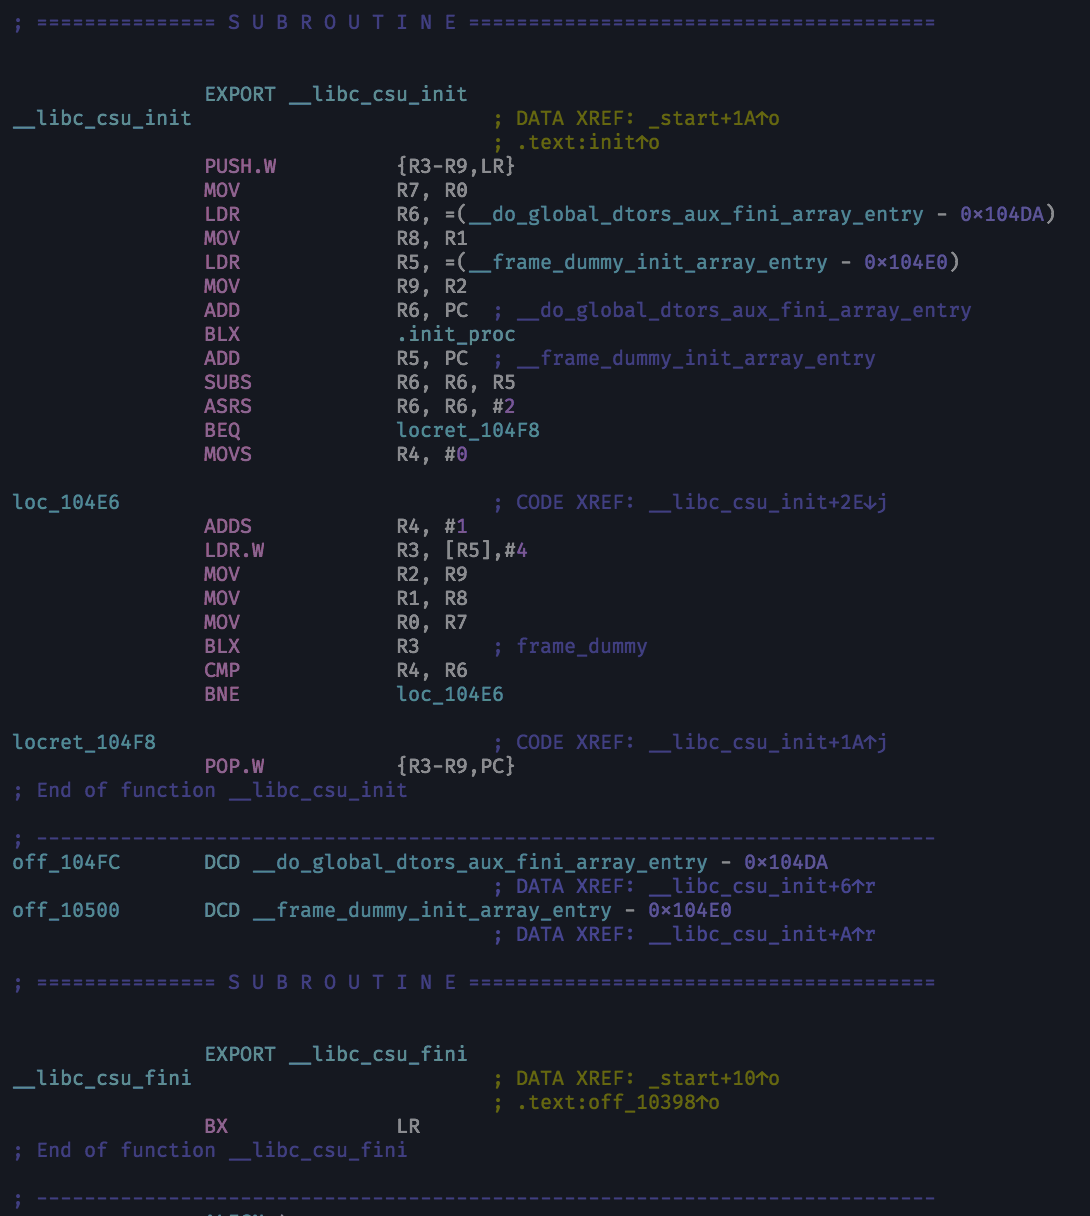
\includegraphics[width=0.4\paperwidth, height=\paperheight]{rpisec_background2.png}
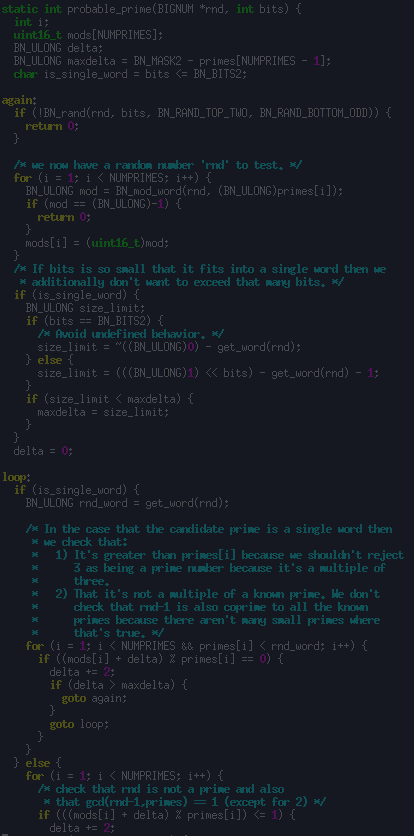
\includegraphics[width=0.4\paperwidth, height=\paperheight]{../rsa_2019_10_29/probable_prime2.png}
}}
}

\begin{document}
\maketitle

\begin{frame}[fragile]
\frametitle{Overview}
\begin{itemize}
\item What are SAT/SMT/Z3?
\item Solving MBE lab1A with Z3
\item Solving a Cyberseed RE challenge with Z3
\end{itemize}
\end{frame}

\begin{frame}[fragile]
\frametitle{What is SAT?}
\begin{itemize}
\item SAT is the boolean SATisfiability problem
\item e.g. "Does the formula $(x \lor \neg y \lor z) \land (\neg x \lor y)$ have a satisfying assignment?"
\item Brute forceable in $O(2^n)$ by trying all combinations of $\{0,1\}$ for all variables
\item NP-Complete 
\begin{itemize}
\item Not known to be subexponentially solvable in general
\item Many problems expressible as SAT
\end{itemize}
\end{itemize}
\end{frame}

\begin{frame}[fragile]
\frametitle{What is SMT?}
\begin{itemize}
\item SMT is Satisfiability Modulo Theories
\item "Does $(f(x,y) \lor z) \land (\neg g(x) = f(x, x))$ have a satisfying assignment?" (QF-EUF)
\item "Does $2*x+y \le z \land x+3*y \ge z$ have a satisfying assignment" (QF-LIA)
\item Allows more compact translation of problems, e.g.
\begin{itemize}
\item $x = 1 \lor x = 2 \lor x = 3 \lor \hdots \lor x = 99 \lor x = 100$ (SAT)
\item $1 \le x \land x \le 100$ (SMT)
\end{itemize}
\item Also NP-Complete
\end{itemize}
\end{frame}

\begin{frame}[fragile]
\frametitle{Why are SAT/SMT useful if they're hard to solve quickly?}
\begin{itemize}
\item Not all problems are as hard as the hardest ones
\begin{itemize}
\item 2-SAT (each clause having at most 2 variables) is polytime solvable
\item Monotone circuits (only ANDs and ORs, no NOTs) are polytime solvable
\end{itemize}
\item It's often possible to prune the search space 
\begin{itemize}
\item e.g. $x \lor \varphi(a, b, c, \hdots)$ is solvable regardless of $\varphi$ because $x=1$ cancels out that subterm
\end{itemize}
\item Algorithms like DPLL and CDCL make use of partial structure to solve some instances faster than others
\item SMT can make use of the rules for the extra types of symbols to prune the search space at a higher level
\end{itemize}
\end{frame}

\begin{frame}[fragile]
\frametitle{What is Z3?}
\begin{itemize}
\item SAT \& SMT solver developed and maintained by Microsoft Research
\item Libre and Open Source (MIT Licensed)
\item C++, with python bindings (\verb|pip install z3-solver|)
\item Based on the CDCL algorithm
\end{itemize}
\end{frame}

\begin{frame}[fragile]
\frametitle{Using Z3 on small examples}
\begin{itemize}
\item $(x \lor \neg y \lor z) \land (\neg x \lor y)$
\item \begin{Verbatim}[fontsize=\scriptsize, frame=single]
import z3
solver = z3.Solver()
x, y, z = z3.Bools('x y z')
solver.add(z3.And(z3.Or(x, z3.Not(y), z), z3.Or(z3.Not(x), y)))
if solver.check().r == 1:
    print(solver.model())
\end{Verbatim}
\item $2*x+y \le z \land x+3*y \ge z \land z > 1$
\item \begin{Verbatim}[fontsize=\scriptsize, frame=single]
import z3
solver = z3.Solver()
x, y, z = z3.Ints('x y z')
solver.add(2*x+y <= z)
solver.add(x+3*y >= z)
solver.add(z > 1)
if solver.check().r == 1:
    print(solver.model())
\end{Verbatim}
\end{itemize}
\end{frame}

\begin{frame}[fragile]
\frametitle{MBE Lab1A - Just Running It}
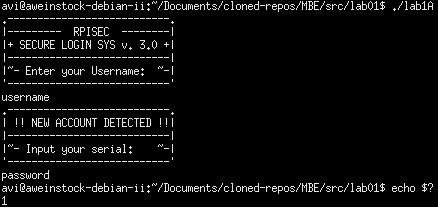
\includegraphics[width=0.9\paperwidth]{pictures/mbe_lab1a_dynamic_fail_cropped.png}
\end{frame}

\begin{frame}[fragile]
\frametitle{MBE Lab1A - Username Entry}
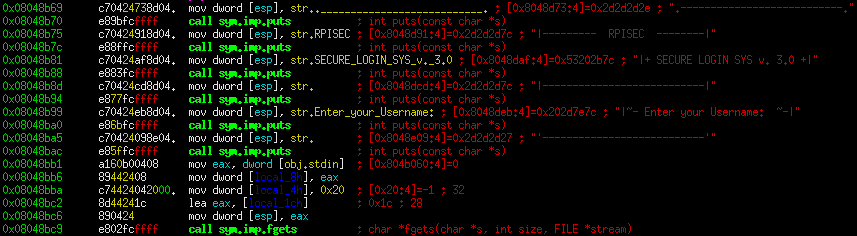
\includegraphics[width=0.9\paperwidth]{pictures/intel/mbe_lab1a_username_entry.png}
\end{frame}

\begin{frame}[fragile]
\frametitle{MBE Lab1A - Serial Entry}
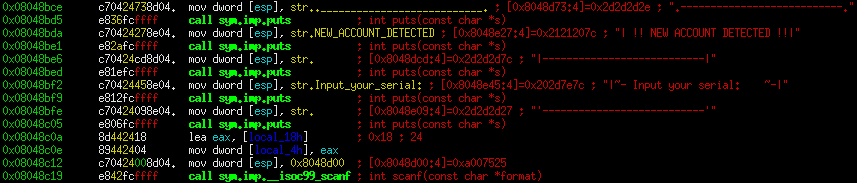
\includegraphics[width=0.9\paperwidth]{pictures/intel/mbe_lab1a_serial_entry.png}\\
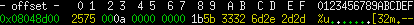
\includegraphics[width=0.9\paperwidth]{pictures/mbe_lab1_scanf_arg_cropped.png}
\end{frame}

\begin{frame}[fragile]
\frametitle{MBE Lab1A - Calling the authentication routine}
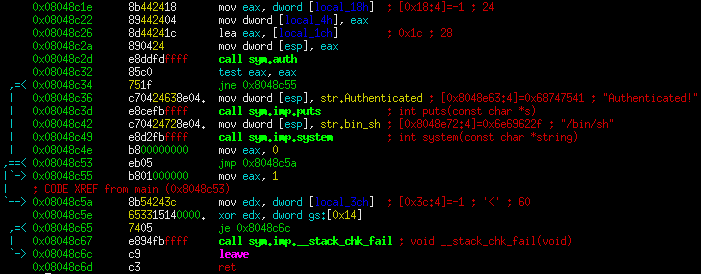
\includegraphics[width=0.9\paperwidth]{pictures/intel/mbe_lab1a_call_auth.png}
\end{frame}

\begin{frame}[fragile]
\frametitle{MBE Lab1A - auth() 1/6: String processing and antidecomp}
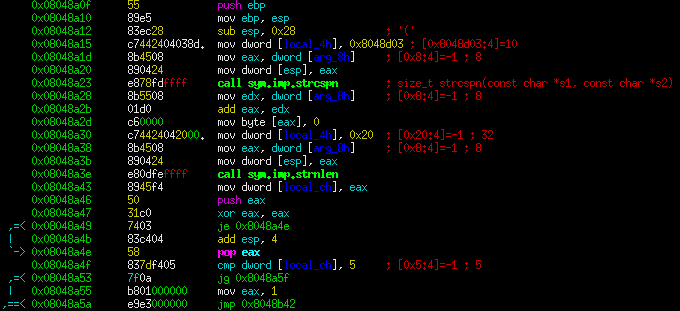
\includegraphics[width=0.9\paperwidth]{pictures/intel/mbe_lab1a_auth_chunk1.png}
\end{frame}

\begin{frame}[fragile]
\frametitle{MBE Lab1A - auth() 2/6: Antidebugging with ptrace}
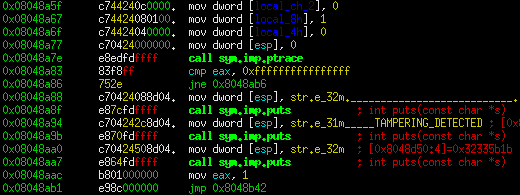
\includegraphics[width=0.9\paperwidth]{pictures/intel/mbe_lab1a_auth_chunk2.png}
\end{frame}

\begin{frame}[fragile]
\frametitle{MBE Lab1A - auth() 3/6: Pre-loop math}
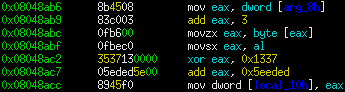
\includegraphics[width=0.9\paperwidth]{pictures/intel/mbe_lab1a_auth_chunk3.png}
\end{frame}

\begin{frame}[fragile]
\frametitle{MBE Lab1A - auth() 4/6: Loop header, restricting chars}
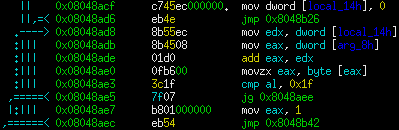
\includegraphics[width=0.9\paperwidth]{pictures/intel/mbe_lab1a_auth_chunk4.png}
\end{frame}

\begin{frame}[fragile]
\frametitle{MBE Lab1A - auth() 5/6: Loop body, much math}
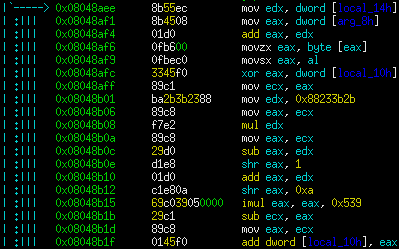
\includegraphics[width=0.9\paperwidth]{pictures/intel/mbe_lab1a_auth_chunk5.png}
\end{frame}

\begin{frame}[fragile]
\frametitle{MBE Lab1A - auth() 6/6: Loop footer, return targets}
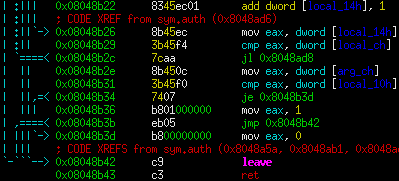
\includegraphics[width=0.9\paperwidth]{pictures/intel/mbe_lab1a_auth_chunk6.png}
\end{frame}

\begin{frame}[fragile]
\frametitle{MBE Lab1A - Z3ing auth() 1/?: Setting up variables}
\begin{Verbatim}[fontsize=\scriptsize, frame=single]
import z3
solver = z3.Solver()
wanted_length = 6
assert wanted_length > 5 # checked at 0x08048a4f
sym_username = [z3.BitVec('x{i}'.format(i=i), 8) for i in range(wanted_length)]
sym_serial = z3.BitVec('serial', 32)
\end{Verbatim}
\begin{itemize}
\item 8-bit entries for each character
\item 32-bit serial number
\item Concrete input length: \verb|z3.Array| exists, but is more expensive
\item Only use \verb|z3.Array| if you need symbolic indexing
\end{itemize}
\end{frame}

\begin{frame}[fragile]
\frametitle{MBE Lab1A - Z3ing auth() 2/?: Translating the pre-loop math}
\begin{Verbatim}[fontsize=\scriptsize, frame=single]
eax = sym_username[3]
eax ^= z3.BitVecVal(0x1337, 32)
eax += z3.BitVecVal(0x5eeded, 32)
local_10h = eax
\end{Verbatim}
\begin{itemize}
\item We're wrapping concrete values in \verb|z3.BitVecVal| so that wrapping/truncation happens the x86 way
\item If we wre using python longs here, we'd have to manually mask them back into range
\end{itemize}
\end{frame}

\begin{frame}[fragile]
\frametitle{Resources}
\begin{itemize}
\item \verb|https://github.com/Z3Prover/z3/|
\item \verb|https://pypi.org/project/z3-solver/|
\item \verb|https://rise4fun.com/Z3/tutorialcontent/guide|
\item \verb|https://en.wikipedia.org/wiki/Satisfiability_modulo_theories|
\item \verb|https://github.com/RPISEC/MBE|
\end{itemize}
\end{frame}
\end{document}
